%--- 11 ----------------------------------------------------------
\item\qouv{Quelles sont les différentes étapes de l’appel d’un service web ?}
{
L'architecture orientée-services (SOA) est un modèle d'architecture dans lequel les composants fournissent des services à des consommateurs (autres services où utilisateurs). Un service consiste en une \textbf{fonction bien définie} (avec ses limitations fonctionnelles et un rôle spécifique), \textbf{indépendante} et \textbf{mise à disposition} selon un "contrat" qui définit son utilisation.
\paragraph{}
Un service n'a pas d'état, il ne retient pas d'information sur les données qu'il traîte. Ainsi par exemple, un service de login permet d'authentifier un user mais il n'a pas conscience des users connectés, cela relève de la responsabilité de l'application.
\paragraph{}
Les données et les services, qui représentent la logique du système, sont \textbf{distribués}. Les services communiquent entre eux via des protocoles d'échanges de messages qui \textbf{suivent des standards}, ce qui assure le découplage et les rend facilement \textbf{réutilisables} pour former de nouveaux processus.
\paragraph{}
Les caractéristiques que doit satisfaire une telle architecture sont les suivantes:
\begin{enumerate}
\item avoir des \textcolor{ltred}{\textsc{frontières bien définies}}: 1 service = 1 fonctionnalité -> ensemble d'opérations définies
\item \textcolor{ltred}{\textsc{autonomie}} des services: les services doivent être indépendant, ce qui induit un faible couplage
\item les services partagent leur \textcolor{ltred}{\textsc{contrat}}: description du service -> ses fonctions et son utilisation
\item les services sont \textcolor{ltred}{\textsc{compatibles suivant des politiques}}: fonctionnalités du services changent selon contexte  (mise en page suivant navigateur web, gratuit/payant suivant utlisateur,...)
\end{enumerate}

\paragraph{}
Un "\textit{service web}" est un protocole qui permet à des applications, aux fonctionnalités diverses, d'échanger des données entre elles, il implémentate une architecture SOA . La figure \cite{appel-service-web} décrit la procédure d'appel d'un service web.
\paragraph{}
Différentes technologies sont utilisées par les services webs:
\begin{enumerate}
\item \textcolor{ltred}{\textsc{HTTP(s)}} (\textit{\textbf{H}yper\textbf{T}ext \textbf{T}rasnfert \textbf{P}rotocol \textbf{S}ecure}): communications
\item \textcolor{ltred}{\textsc{XML}} (\textit{e\textbf{X}tensible \textbf{M}arkup \textbf{L}anguage}) ou \textcolor{ltred}{\textsc{JSON}} (\textit{\textbf{J}ava\textbf{S}ript \textbf{O}bject \textbf{N}otation}): construction messages
\item \textcolor{ltred}{\textsc{WSDL}} (\textit{\textbf{W}eb \textbf{S}ervices \textbf{D}escription \textbf{L}anguage}): description précise des signatures (\textit{quoi}, \textit{où}, \textit{comment}) des services invoquables
\item \textcolor{ltred}{\textsc{UDDI}} (\textit{\textbf{U}niversal \textbf{D}escription, \textbf{D}iscovery, and \textbf{I}ntegration}): annuraire des services disponibles, protocole d'enregistrement des services
\item \textcolor{ltred}{\textsc{SOAP}} (\textit{\textbf{S}imple \textbf{O}bject \textbf{A}ccess \textbf{P}rotocol}): protocole d'invocation des messages
\end{enumerate}

\begin{figure}[h!]
\center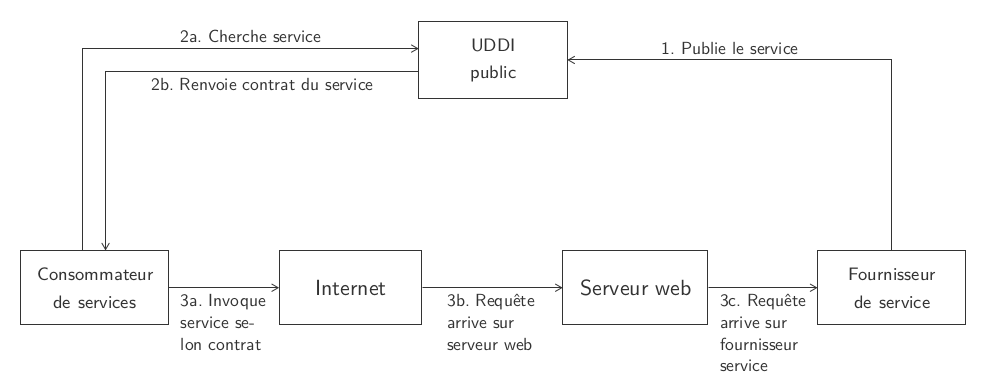
\includegraphics[scale=.4]{images/services-web}
\caption{Protocole d'appel d'un service web \cite{ref1}}
\label{appel-service-web}
\end{figure}

\paragraph{}Description des étapes:
\begin{enumerate}
\item \textcolor{ltred}{\textsc{publication du service}}: le fournisseur de service rapporte à l'annuaire sa présence. Autrement dit, il se fait connaître sur le réseau.
\item \textcolor{ltred}{\textsc{Recherche de service}} et \textcolor{ltred}{\textsc{envoie du contrat}}: Le consommateur interroge le répertoire de services pour prendre connaissance des services disponibles et connaître leurs contrats, c'est-à-dire la façon de les utiliser. Cette étape est nécessaire uniquement lors de la première utilisation d'un service (ou de temps en temps par après pour vérifier d'éventuelles mises à jour).
\item \textcolor{ltred}{\textsc{invocation du service}}: le consommateur fait appel au service selon les conditions définies par le contrat. La requête passe par le réseau Internet et arrive au serveur qui contient le code source pour exécuter le service.
\item \textcolor{ltred}{\textsc{réponse du service}}: le service effectue ses opérations et retourne une réponse au consommateur.
\end{enumerate}
}


%--- 12 ----------------------------------------------------------
\item\qouv{Expliquez brièvement les six contraintes d’une architecture REST ?}
{
REST (\textit{\textbf{RE}presentation \textbf{S}tate \textbf{T}ransfer}) est une architecture dédiée au développement de services web. Il s'agit d'une \textbf{collection de principes/contraintes/conventions} qui ne consitutent pas des standards (ce n'est pas une technologie en soi!) Autrement dit, leur utilisation n'est pas obligatoire pour l'implémentation d'un tel service.
\paragraph{}
L'architecture REST est définie par 6 principes:
\begin{enumerate}\setlength{\itemsep}{.3em}
\item\textcolor{ltred}{\textsc{uniform interface}}: interface uniforme entre le client et le serveur où les ressources sont identifiées par un \textbf{URI} (\textit{\textbf{U}niform \textbf{R}essource \textbf{I}dentifier}). Les requêtes reposent sur l'utilisation du \textbf{protocole HTTP} avec une hiérarchie des ressources et des \textit{query string} uniquement en tant que filtres (\textit{ex: \textcolor{dkyellow}{GET} http://www.example.com/\textcolor{purple}{customers/1234/orders}\textcolor{dkgreen}{?offset=0\& limit=25}}).

\item\textcolor{ltred}{\textsc{state less}}: le service n'a pas d'état, il ne conserve pas l'état des ressources, il n'existe donc pas de session entre le serveur et le client. C'est la \textbf{requête} (donc responsabilité côté client/application) qui \textbf{contient toute l'information} nécessaire à son traitement.\paragraph{}Ce principe permet de facilement déployer le service sur différents serveurs, le client pouvant alors être indifféremment redirigé vers l'un d'entre eux. En revanche, cela implique une mise en place correcte de la sémantique de l'application, puisque le serveur perd une partie du contrôle.

\item\textcolor{ltred}{\textsc{cacheable}}: possibilité de mettre une réponse en cache (côté serveur ou client) pour \textbf{augmenter les performances}. Ces informations en mémoire évitent de formuler des requêtes inutilement ou de traiter des requêtes identiques, mais avec un risque que celles-ci soient obsolètes (à contrôler).

\item\textcolor{ltred}{\textsc{client-serveur}}: \textbf{séparation précise des responsabilités} du serveur et du client, ce qui leur permet d'évoluer indépendamment.

\item\textcolor{ltred}{\textsc{layered system}}: définitions de \textbf{couches}, de telle sorte qu'une couche n'ait accès qu'à des composant d'une couche avec laquelle elle communique directement.

\item\textcolor{ltred}{\textsc{code on demand}}: le serveur envoie le code (JavaScript,...) au client de telle sorte qu'il puisse faire varier les fonctionnalités du service en fonction du client. \textbf{Variation dynamqiue du service} en fonction du contexte d'utilisation. 
\end{enumerate}
\paragraph{}
Lorsque les 6 contraintes sont implémentées, on parle alors d'architecture \textit{RESTful}.

\paragraph{}
Les avantages d'une telle architecture sont les suivants:
\begin{itemize}\setlength{\itemsep}{.2em}
\item[\textcolor{dkgreen}{\ding{52}}]répartition des requêtes et meilleure tolérance aux pannes, dus à l'absence d'état et donc la duplication du service
\item[\textcolor{dkgreen}{\ding{52}}]soulagement 
\end{itemize}
}


%--- 13 ----------------------------------------------------------
\item\qouv{Exposez brièvement les différences entre IaaS, PaaS et Saas.}
{}


%--- 14 ----------------------------------------------------------
\item\qouv{Exposez brièvement les différences entre IaaS, PaaS et Saas.}
{}


%--- 15 ----------------------------------------------------------
\item\qouv{Comment se calcule la complexité Fan-in Fan-out et quels sont ses avantages et inconvénients ?}
{La complexité "Fan-in Fan-out" est un \textit{métrique} qui se base sur le flux des données locales (in=params et out=valeurs retour).
\paragraph{}
Deux variantes existent pour calculer cette valeur de complexité:
\begin{enumerate}
\item \textbf{Henry et Kafura}: $HK = Length * (Fan_{in} * Fan_{out})^{2}$
\item \textbf{Shepperd}: $S = (Fan_{in} * Fan_{out})^{2}$
\end{enumerate}

\paragraph{UTILITE [...]}
}


%--- 16 ----------------------------------------------------------
\item\qouv{Définissez les notions de couplage afferent et efferent. Comment construit-on l’instabilité à partir
de ces métriques.}
{}

%--- 17 ----------------------------------------------------------
\item\qouv{Qu’est-ce-que la distance from main sequence et que permet-elle de mesurer ?}
{}

%--- 18 ----------------------------------------------------------
\item\qouv{Définissez brièvement les principes DRY et WET.}
{}

%--- 19 ----------------------------------------------------------
\item\qouv{Définissez le concept d’orthogonalité. En quoi améliore-t-il la qualité d’un logiciel ?}
{}

%--- 20 ----------------------------------------------------------
\item\qouv{Expliquez brièvement le principe du code traçant.}
{}